% THIS IS SIGPROC-SP.TEX - VERSION 3.1
% WORKS WITH V3.2SP OF ACM_PROC_ARTICLE-SP.CLS
% APRIL 2009
%
% It is an example file showing how to use the 'acm_proc_article-sp.cls' V3.2SP
% LaTeX2e document class file for Conference Proceedings submissions.
% ----------------------------------------------------------------------------------------------------------------
% This .tex file (and associated .cls V3.2SP) *DOES NOT* produce:
%       1) The Permission Statement
%       2) The Conference (location) Info information
%       3) The Copyright Line with ACM data
%       4) Page numbering
% ---------------------------------------------------------------------------------------------------------------
% It is an example which *does* use the .bib file (from which the .bbl file
% is produced).
% REMEMBER HOWEVER: After having produced the .bbl file,
% and prior to final submission,
% you need to 'insert'  your .bbl file into your source .tex file so as to provide
% ONE 'self-contained' source file.
%
% Questions regarding SIGS should be sent to
% Adrienne Griscti ---> griscti@acm.org
%
% Questions/suggestions regarding the guidelines, .tex and .cls files, etc. to
% Gerald Murray ---> murray@hq.acm.org
%
% For tracking purposes - this is V3.1SP - APRIL 2009

\documentclass{acm_proc_article-sp}
\usepackage{graphicx}
\graphicspath{ {images/} }

\begin{document}

\title{A Study of Parking Issues on NC State Campus}
%\subtitle{[Data Collection]}

\numberofauthors{4} 
\author{
\alignauthor
Ahmad Saad Khan\\ %\titlenote{Now on postdoctoral fellow at ABC University}\\
       \affaddr{North Carolina State University}\\
       \affaddr{Raleigh NC}\\
       \email{akhan7@ncsu.edu}
\alignauthor
Krishna Agarwala\\
       \affaddr{North Carolina State University}\\
       \affaddr{Raleigh NC}\\
       \email{kagarwa@ncsu.edu}
\alignauthor
Nikhil Raina\\
       \affaddr{North Carolina State University}\\
       \affaddr{Raleigh NC}\\
       \email{nraina@ncsu.edu}
\and % go to new row
\alignauthor
Snehasis Ghosh\\
       \affaddr{North Carolina State University}\\
       \affaddr{Raleigh NC}\\
       \email{sghosh9@ncsu.edu}
}

\date{07 April 2016}


\maketitle
\begin{abstract}
This project report introduces the problem of parking faced in all colleges and universities throughout the United States and also the world at large. There are three solutions presented based primarily on feedback from a focus group comprising of students of North Carolina State University who've helped us in defining the problem. We present the three solutions and analyse all three of them to find the benefits and shortcomings of each of them. We finally draw a conclusion based on the solutions and our own experience working on this project.
\end{abstract}

%A category with the (minimum) three required fields
%\category{H.4}{Information Systems Applications}{Miscellaneous}
%A category including the fourth, optional field follows...
%\category{D.2.8}{Software Engineering}{Metrics}[complexity measures, performance measures]

%\terms{Theory}

%\keywords{Parking Problem, Parking Navigation, Parking slot, Parking management, } % NOT required for Proceedings

% A category with the (minimum) three required fields
%\category{H.4}{Information Systems Applications}{Miscellaneous}
%A category including the fourth, optional field follows...
%\category{D.2.8}{Software Engineering}{Metrics}[complexity measures, performance measures]

%\terms{Theory}

%\keywords{ACM proceedings, \LaTeX, text tagging} % NOT required for Proceedings

\section{Introduction}
Reflecting on former President of University of California, Clark Kerr's words-  "I have sometimes thought of the modern [U.S.] university as a series of individual faculty entrepreneurs held together by a common grievance over parking.", one can draw the conclusion that his words ring painfully true in today's day and age. Without a doubt parking seems to seems to be the most widespread and frustrating problems affecting Colleges and Universities. Rising enrollment numbers are one of the main reasons that so many institutions are facing parking shortages. Enrollment jumped from 14.5 million to 18.2 million between 1997 and 2007 in the United States, putting a severe strain on a service that's already at the breaking point. One could also point to how today's students are products of a "car culture" that urges them to drive to destinations when walking will often suffice. 

To combat this problem, we proposed an automated parking solution, which is an Android application which aims to solve a lot of the problems facing all the stakeholders on college campuses. We have offered 3 different solutions to combat the problems of parking, and they are as follows:

\begin{enumerate}
  \item Standalone NCSU parking application: A user can download the application on their Android phone and it enables them see the percentage of empty space in any of the NCSU parking lots. Using this they have an idea about possible parking spaces or lack-thereof, before they even arrive at the campus.
  \item NCSU Parking App with login and authentication: A user can register and sign up on the same application. By signing up on the app a user can also "favorite" a particular parking slot on campus, maybe one where they have to park each day and they can get real time notification on their phone indicating that the parking spot is currently full.
  \item  Parking Management System: A registered user can also use the same application as a central hub of parking management system. The user can register their car in this system using their car's number plate. This connects to the central transportation centre of NCSU so essentially the user has registered his/her car with the NCSU transport office. If the car happens to be parked illegally on campus and a fine is issued on the car or if the car is being towed the transport office can send a real-time notification to the user about the traffic violation being issued or the fact that the car is being towed. This system can also keep track of the fines collected on a particular car based on their number plate and a user can pay their fines from within the application by collecting to the NCSU Shibboleth server for authentication and payment of the fine.
\end{enumerate}

Thus these 3 solutions aim to provide a holistic approach to solving the parking problem on NCSU campus.

\section{Research}
A very important part of this study was to collect the general consensus of public with respect to the issues and data regarding the problems that are faced when handling this subject. We adopted three different approaches : Personal Interviews, Survey, and going through the public information made available by American Planning Association\cite{APA} and other white papers.

\subsection{Personal Interviews}
We visited different parking locations within the campus and spoke to various students, faculty and staff. The parking spots covered in this task were: Alliance Deck, Poulton Deck, and Coliseum Deck. Talking to people first hand about the problems faced by them helped us formalize the problem in a more structured way. It also made us realise that parking spot availability is not the only issue faced by the users. The parking management system seems to have major communication gap with the users. We discussed various solutions to the problems and asked them to grade them. 

Initially, we had thought of providing a solution only for finding available parking slots. However, this exercise helped us realise that along with this, parking management system also needs to be streamlined to make it easier for new users to carry out administrative tasks. As this application is only available through a web portal, users do require a mobile application to handle the same. This helped us reframe our understanding of the requirement and we structured the online survey form accordingly.

\subsection{Survey} 
We created a survey\cite{gooform} where we had formulated a set of questions and presented it to people to record their responses. This survey was circulated to our colleagues in NCSU via direct e-mails, Facebook, Whatsapp and other social networking sites.


\begin{itemize}
    \item Do you own a car which you bring regularly to campus?
    \begin{itemize}
        \item Yes
        \item No
    \end{itemize}
    
    \begin{figure}[h!]
        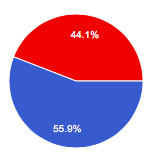
\includegraphics{Q1}
        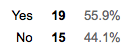
\includegraphics[height = 1cm]{Q1_1}
        \caption{Percentage distribution for question 1}
        \label{fig:Q1_1}
    \end{figure}
    
    This question served two purposes, it acted as a filter to identify the outliers i.e. people who don\textsc{\char39}t own cars. It also served the purpose of identifying the issues faced by people who regularly commute to campus via car versus the people who rarely do.
    
    \item What do you think is the biggest problem associated with bringing a car to campus?
    \begin{itemize}
        \item Cost of parking
        \item Finding a parking spot near your destination
        \item Other
    \end{itemize}
    
    \begin{figure}[h!]
        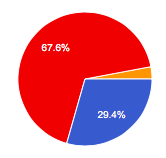
\includegraphics{Q2}
        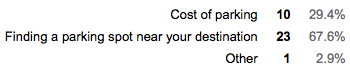
\includegraphics[width=8cm, height = 1cm]{Q2_2}
        \caption{Percentage distribution for question 2}
        \label{fig:Q2_2}
    \end{figure}
    
    This question was directly aimed at figuring out the core problem. As economics of parking plays an important role for users (mainly students), this question helped in grading the importance of the given two factors.

    \item Would you prefer a mobile app for parking management system that can track your tickets/fines as well?
    \begin{itemize}
        \item Yes
        \item No
    \end{itemize}
    
    \begin{figure}[h!]
        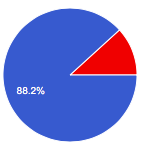
\includegraphics{Q_3}
        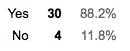
\includegraphics[height = 1cm]{Q3_3}
        \caption{Percentage distribution for question 3}
        \label{fig:Q3_3}
    \end{figure}
    
    This question was added to the survey after the personal interviews, as we realized that people who were new to the campus and didn't\textsc{\char39}t bring car regularly to campus are more inclined towards having a mobile app for NCSU Transport Management. Since they were in the process of getting their cars registered with the university they were more inclined towards the initial setup. Compared to this people who brought their cars regularly to campus were more inclined towards a Car Parking finder App.
    
    \item Would you like an automatic search and payment option for parking?
    \begin{itemize}
        \item Yes
        \item No
    \end{itemize}
    
    \begin{figure}[h!]
        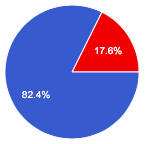
\includegraphics{Q4}
        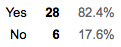
\includegraphics[height = 1cm]{Q4_4}
        \caption{Percentage distribution for question 4}
        \label{fig:Q4_4}
    \end{figure}
    
    This question was also added after personal interviews were conducted. We felt from the tone of people that this was something that everybody using the parking system needed.\\
    
    \item Would you like to include options for parking rule violations reporting?
    \begin{itemize}
        \item Yes
        \item No
    \end{itemize}
    
    \begin{figure}[h!]
        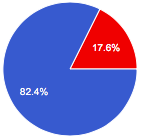
\includegraphics{Q5}
        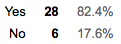
\includegraphics[height = 1cm]{Q5_5}
        \caption{Percentage distribution for question 5}
        \label{fig:Q5_5}
    \end{figure}
    
\end{itemize}

The following questions were subjective questions which were included to understand any other kind of issue which we would have missed in the personal interviews or the survey.

\begin{itemize}
    \item Can you share some horror story you or someone you know faced while bringing a car to campus?
    
    \begin{itemize}
        \item Getting a ticket on parking in a wrong lot.
        \item Getting towed for running in to turn in a paper.
        \item It was too expensive to park on campus so a friend of mine has to park off campus and take a bus despite owning a car.
        \item I know a friend of mine who did not have a pass, ended up paying so much for few hours and bought a parking permit the same day.
    \end{itemize}
    
    \item Would you like to share your overall experience with bringing a car to campus?
    
    \begin{itemize}
        \item Takes a lot of time and effort from my day to get to class on time due to lack of AFFORDABLE parking.
        \item It is annoying to park not only because of the limited parking available (especially overnight) but also the high prices that come with it.
        \item The main thing I am frustrated with is trying to get a parking permit for Dan Allen. Even though I have enough credit hours now, it still won\textsc{\char39}t let me even get on the wait list until next school year.
        \item It has been mostly fine so far, really the only annoying thing is not knowing all of the rules regarding parking.
        \item HORRIBLE. There are so few places to park anywhere temporarily
        \item The parking fee is expensive and the parking lot is hard to find. That is why I only take school bus to school.
        \item It is normally ok if you come early in the morning, but it is a hassle at other times of the day to try to find a spot that is not on the roof of the deck and the traffic in the deck is awful too
        \item Good and expensive. I always find a spot very fast.
    \end{itemize}

\end{itemize}

These responses helps us understand that a more streamlined application is required which can help people identify correct parking spots, handle towing issues, and realizing parking costs accurately.

\section{Proposed Solutions}
Now that the problem has been extensively examined and there is little doubt of the scope of the problem, an all-in-one solution is needed to address all the problems which have been identified. Mobile phones have become ubiquitous and their computation power as well as usability have reached the point that a lot of users rely solely on their mobile devices for most of their daily task. Hence for maximum reachability and ease of use from a user's point of view, building an Android application was determined to be the best solution. During the course of the project development phase, we have developed a simple Android application which aims to automate the parking system on NCSU campus.


\section{Observations}
The survey included in this project yielded very important results giving insight into the user demand from a parking solution. The literature survey indicated the area of research which is being done around the world and also the problems faced and the advantages and disadvantages of the solutions proposed. The online survey included responses from 34 people through a Google survey form\cite{gooform} in which 55.9\textsc{\char37} (19 people) owned a car which they regularly brought to campus and 44.1\textsc{\char37} (15 people) did regularly bring a car to campus but used a car occasionally. Other responses include 67.6\textsc{\char37} of the people surveyed indicating that finding a parking spot near their destination was the biggest problem they faced when bringing a car on campus. Nearly 80\textsc{\char37}-90\textsc{\char37} of the people agreed that a solution for this issue needs to have the abilities to track the fines associated with your car and automate search and payment options for parking as well as reporting parking rule violations reporting. Some real-life experiences shared by the people included getting ticketed for parking in a wrong lot, getting towed for neglecting to pay adequate amount for parking due to paper submission, and the increasing cost of parking deterring owners of cars to bring them on campus. A majority of the people felt that the cost of parking is the number one problem faced for students and they should have more options for parking with reasonable parking rates. Other problems faced by students are the lack of clear cut rules regarding parking and the confusion regarding the lots for which their parking passes are valid. This problem was mainly seen in people who are new to University or are occasional users of car for transit.

If we try to classify these problems on a high level we could classify them into two groups : Group-1 refers to the problems people face while finding the parking spot, Group-2 refers to the administrative problems faced by people who own cars. Primary need for people belonging to Group-1 is to have a robust, Google Maps like application, that they can use on handheld devices to locate available parking spots on campus. And primary need for people belonging to Group-2 is to have an application that lets them solve the administrative requirements like registration, payment of fine etc on the fly without them having to open a Desktop/Laptop and login to NCSU transportation website.


\section{Conclusion}
It is clear from the survey and literature review that parking troubles on campus are increasingly becoming a real worry for all of the members of the university. The need of the hour is to produce a parking solution that not only informs about free parking spaces but also lists out the cost of parking in different lots and keeps a track of the parking violations and fines incurred on a user\textsc{\char39}s car. There are both software as well as hardware solutions to address the problem. The hardware solution requires more infrastructure and an overhaul of the university parking system but is likely to produce more long lasting results. This can include putting motion sensors on parking lots to indicate if a lot is vacant or not. The software solution includes the use of scanners to scan the license plate of a car in case of violations or fines and collecting this data on a central server. This can trigger several actions like setting off an alert on a driver\textsc{\char39}s smartphone informing him/her about the violation. Other solutions include an algorithm to calculate the free parking spaces depending on two key factors - the distance between the driver\textsc{\char39}s destination and the parking lot, and the cost of parking and budget constraints of the driver. Further research needs to be done to present a parking solution encompassing all these factors and coming up with a viable solution.



\begin{thebibliography}{10}
\bibitem{gooform}
Google form on which observations are based:
\textit{http://bit.ly/1Pc3dnl}.
 
\bibitem{Giuffre} 
T. Giuffre, S.M. Siniscalchi, G. Tesoriere
\textit{A novel architecture of parking management for smart cities}.
Procedia - Soc. Behav. Sci., 53 (2012), pp. 16-28

\bibitem{Arnott} 
R. Arnott, T. Rave, R. Schöb
\textit{Arnott et al. Alleviating Urban Traffic Congestion}.
MIT Press (2005)

\bibitem{Soup} 
D. Soup
\textit{Cruising for parking}.
Access, 30 (2007), pp. 16-22

\bibitem{Caliskan} 
Caliskan, M., Barthels, A., Scheuermann, B., Mauve, M.
\textit{Caliskan et al. Predicting Parking Lot Occupancy in Vehicular Ad Hoc Networks}.
IEEE 65th Conference on Vehicular Technology, 2007

\bibitem{Caicedo} 
F. Caicedo
\textit{Real-time parking information management to reduce search time, vehicle displacement and emissions}.
Transport. Res. Part D: Transp. Environ., 15 (4) (2010), pp. 228-234

\bibitem{Joseph} 
Joseph, Jeffrey; Patil, Roshan Gajanan; Narahari, Skanda Kumar Kaipu; Didagi, Yogish; Bapat, Jyotsna
\textit{Wireless Sensor Network Based Smart Parking System}.
Sensors  Transducers, Vol. 162 , Issue 1, January 2014, pp. 5-10

\bibitem{Yanfeng} 
Yanfeng Geng, Christos G. Cassandras
\textit{New \textsc{\char34}Smart Parking\textsc{\char34} System Based on Resource}.
Allocation and Reservations; IEEE Transactions on Intelligent Transportation Systems, ISSN 1524-9050, 2013, Volume 14, Issue 3, pp. 1129 - 1139

\bibitem{Pham} 
Pham, Thanh Nam; Tsai, Ming-Fong; Nguyen, Duc Binh; Dow, Chyi-Ren; Deng, Der-Jiunn
\textit{A Cloud-Based Smart-Parking System Based on Internet-of-Things Technologies}.
IEEE Access, EISSN 2169-3536, 2015, Volume 3, pp. 1581 - 1591

\bibitem{APA}
American Planning Association - Planning Advisory Services
\textit{Parking Problems}.
http://bit.ly/23FDH3q

\end{thebibliography}



%\bibliographystyle{abbrv}
%\bibliography{sample}

%\balancecolumns 

\end{document}
